\chapter{ Констукторский раздел}
\label{cha:design}

В данном разделе мы рассмотрим схемы вышеизложенных алгоритмов.

%!!! В цикле скругление убрать и начало поменять

\section{Разработка алгоритмов}

% !!! Написать до каждой схемы , что вот на этой рис. показано вот это. OK

% !!! Схема алгоритма поиска. OK.

На рис. (\ref{fg:ref1}) представлен алгоритм поиска расстояние Левенштейна.

\begin{figure}[ht!]
	\centering{
		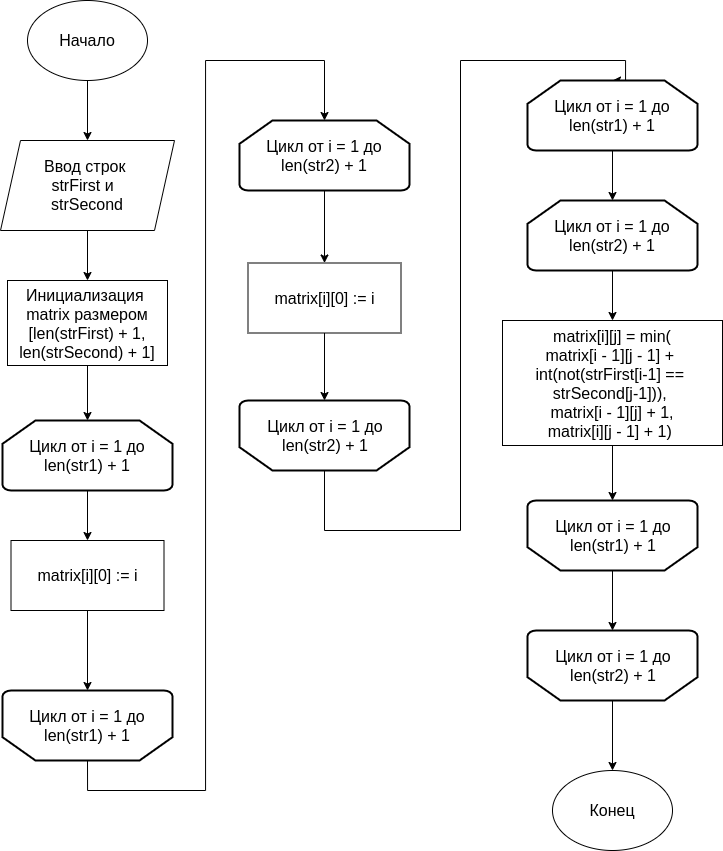
\includegraphics[width=0.6\textwidth]{img/diagramLev.png}
		\caption{Схема алгоритма поиска расстояния Левенштейна}
		\label{fg:ref1}}
\end{figure}

На рис. (\ref{fg:ref2}) представлен алгоритм поиска расстояние Дамерау-Левенштейна.

\begin{figure}[ht!]
	\centering{
		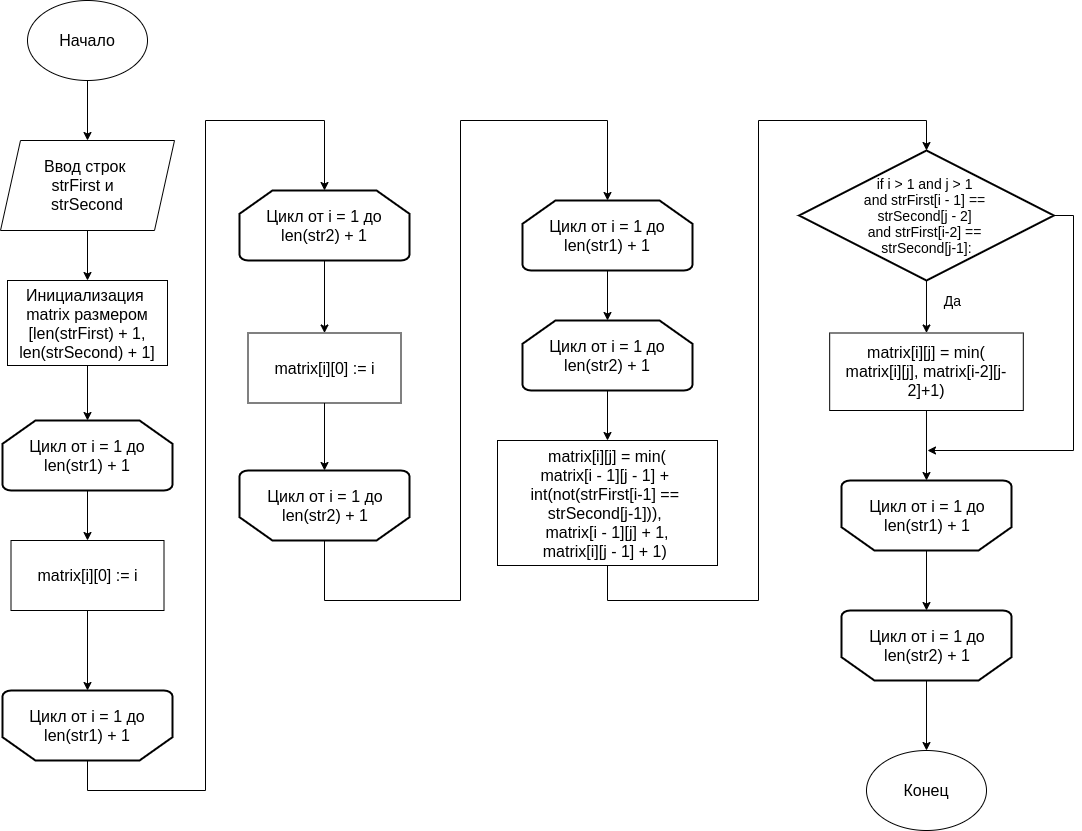
\includegraphics[width=1\textwidth]{img/diagramDamLev.png}
		\caption{Схема алгоритма поиска расстояния Дамерау-Левенштейна}
		\label{fg:ref2}}
\end{figure}

% !!! В рекурсивном алг написать комментарий, что это метод и его название (приделать это к началу схемы) OK

На рис. (\ref{fg:ref3}) представлен рекурсивный алгоритм поиска расстояния Левенштейна.

\begin{figure}[ht!]
	\centering{
		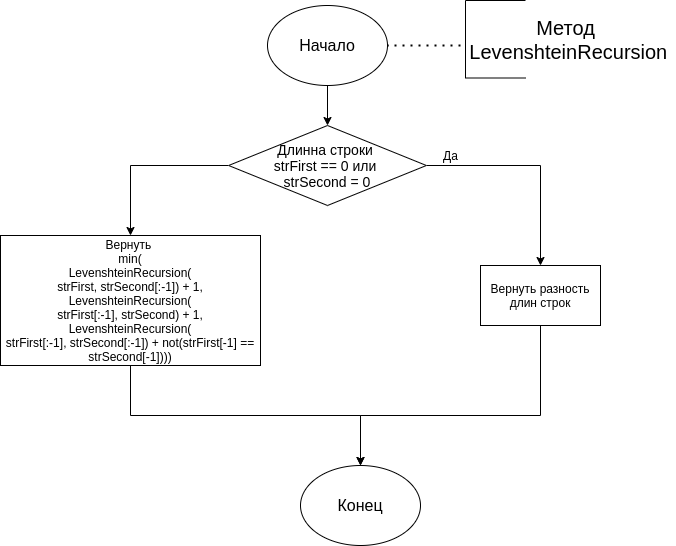
\includegraphics[width=0.8\textwidth]{img/diagramLevRec.png}
		\caption{Схема рекурсивного алгоритма поиска расстояния Левенштейна}
		\label{fg:ref3}}
\end{figure}

\section{Вывод}

В данном разделе мы рассмотрели схемы алгоритмов Левенштейна (\ref{fg:ref1}). и Дамерау-Левенштейна (\ref{fg:ref2}).






